\documentclass{article}
\usepackage{graphicx} % Required for inserting images
\usepackage[numbers]{natbib} % Numeric references
\usepackage{hyperref}
\usepackage[utf8]{inputenc}
\usepackage{multirow}
\usepackage{booktabs}
\usepackage{float}



%\usepackage[ backend=biber, style=numeric, ]{biblatex}

\hypersetup{
    colorlinks=true, % Enable colored links
    linkcolor=black, % Color for internal links (sections, pages)
    citecolor=black, % Color for citation links
    urlcolor=black, % Color for external links (URLs)
    filecolor=black % Color for file links
}

\title{Flow Matching vs Diffusion Models: A Comparative Study}
\author{Sebastian Andersson \and Lo Heander \and Andreas Bexell}
\date{June 2025}

\begin{document}

\maketitle

\section{Introduction}

For this project, we choose to implement and evaluate flow matching and diffusion model families. These model families are particularily interesting to compare since they can both be used for image generation and be trained on the same datasets making direct performance and result comparisons possible. Their internal neural network architectures are also similar, but they use very different loss functions and strategies for training the networks. Because of this, we expect both strong similarities in for example network complexity, training time and accuracy, but also interesting differences in the resulting data generated from the same inputs.

\section{Model Families}

\subsection{Diffusion}

Diffusion models is a type of deep generative models that has found many applications recently, especially for image generation. The models are based on two diffusion stages. In the \emph{forward diffusion stage}, normally distributed noise is incrementally added to the training data, until the original data is entirely obscured by noise. In the next stage, the \emph{reverse diffusion stage}, the model is trained to recover the original data from the noisy data at each step. Ultimately, this enables the model to generate new data from pure noise. If conditioned with an additional label or prompt during training, the model can become able to generate data from a combination of noise and instruction~\cite{croitoru2023diffusion,yang2023diffusion}. Diffusion models have applications not only in image generation, but also text, speech, biology and healthcare~\cite{cao2024survey}.

Croitoru et al. conducts a survey on how diffision models apply to computer vision use-cases~\cite{croitoru2023diffusion}. To start with, they outline three main categories of diffusion models:

\paragraph{Denoising Diffusion Probabalistic Models (DDPMs)} 
DDPMs model a probability distribution of the applied noise in the latent space of the neural model. DDPMs typically require many, in the order of 1000 or more, discrete steps when adding the noise. It uses a stochastic sampling strategy that, while requiring many steps, can lead to more diverse outputs. They are very flexible and can be optimized using a variety of different noise schedules and loss functions.

\paragraph{Noise Conditioned Score Networks (NCSNs)} 
Estimates a score function $\nabla_x \log p_t(x)$ at each noise level to determine the direction of lower noise magnitude. The model trains to minimize the loss over several noise levels, and uses the score function to to simulate differential equations that can apply the noise in reverse, that is, to remove the noise.

\paragraph{Stochastic differential equations (SDEs)} 
Stochastic differential equations (SDEs) model diffusion as a continuous-time process, providing a unifying framework that generalizes both DDPMs and NCSNs. In this approach, the forward diffusion is described by a stochastic differential equation, and the model learns to reverse this process by estimating the score function at each time step. This continuous formulation allows for flexible noise schedules and improved theoretical understanding, bridging the gap between discrete and continuous generative modeling~\cite{song2020score}.


\subsection{Flow matching}

Unlike diffusion models, flow matching models do not use noise injection, and so does not work with denoising as such. Rather, flow matching models take inspiration from fluid dynamics and use a neural network to simulate a vector field that matches the flow between distributions~\cite{holderrieth2025introduction}. This allows flow matching models to train with fewer steps~\cite{kornilov2024optimal} and still potentially be faster and more stable than diffusion models~\cite{lipman2022flow}, since they are deterministic and seeks to follow an optimal transportation path. 

\paragraph{Trajectory flow matching} is a training algorithm for neural differential equation models that require no simulation. It is developed specifically for clinical settings and is able to model processes based on sparse, irregular and noisy data~\cite{zhang2024trajectory}.

\paragraph{Discrete flow matching} is a model designed to perform on discrete sequential data. It is ``a generalization of continuous flow matching and discrete flows'', and seeks to improve performance on tasks such as text generation. The approach is new, and the results are inconclusive, but the authors find it a promising future alternative to autoregressive models~\cite{gat2024discrete}.

\paragraph{Optimal flow matching} seeks to improve inference performance by finding the optimal transport displacements that allow inference in a single step. It does so by simulating straight trajectories that do not require solving differential equations, by, in turn, selecting only vector fields yielding straight paths~\cite{kornilov2024optimal}.

\section{Method}

We begin by implementing two variants of Flow Matching models as well as two variants of Diffusion models. To compare the chosen model families and model variants, we train and evaluate all models on two different datasets:

\paragraph{Two-moons} is a synthetic toy dataset to visualize and benchmark classification and generation, designed to be non-trivial and require higher-order models.

\paragraph{FFHQ} is an open dataset of high-quality images of faces from the online photo-sharing site Flickr. We use it as a traning set and to benchmark the generative models.

\subsection{Metrics}

\paragraph{Wasserstein distance} is a measure of distance between two distributions. Intuitively, it can be understood as the number of steps needed to transform one probability distribution to another. \cite{lil} As a metric, it is intuitive and provides good information about the performance of the model.

\paragraph{Distance entropy} is a measure of the diversity of generated samples. It is calculated as the entropy of the pairwise distances between generated samples, and is used to evaluate how well the model captures the diversity of the training data~\cite{naeem2020reliablefidelitydiversitymetrics}.

\paragraph{Coverage} builds nearest neighbour manifolds around real samples and measures the ratio of the real samples that has fake samples in their neighborhood~\cite{naeem2020reliablefidelitydiversitymetrics}.

\paragraph{Precision} is the probability that a generated artifact falls whithin in the support of the distribution of real artifacts~\cite{kynk2019}.

\paragraph{Fréchet inception distance} (FID) uses the Fréchet distance combined with activations from Inception v3 and is shown to correlate negatively against quality in images~\cite{yu2021frechet}.

\subsection{Variants}

We implement two variants of each model family, Flow Matching and Diffusion. The first variant is a Multi-Layer Perceptron (MLP) model, and the second is a Convolutional Neural Network (CNN) model. The MLP models are used for the Two Moons dataset, while the CNN models are used for the FFHQ dataset.

\subsection{Hyperparameter Optimization}

To optimize the hyperparameters of the models, we use the Optuna library~\cite{akiba2019optuna}. Optuna is a hyperparameter optimization framework that uses a tree-structured Parzen estimator to efficiently search the hyperparameter space. We define a search space for each model and dataset, and use Optuna to find the best hyperparameters for each model.

\section{Results}
We evaluate the models on the Two Moons and FFHQ datasets using the metrics described above. The results are summarized in Table~\ref{tab:results}.


\begin{table}[H]
	\centering
	\caption{Naive and Optuna-optimized hyperparameters for Flow Matching and Diffusion models on Two Moons (MLP) and FFHQ (CNN).}
	\label{tab:results}
	\begin{tabular}{lllrrr}
		\toprule
		\textbf{Model}                 & \textbf{Dataset}                 & \textbf{Hyperparameter} & \textbf{Naïve}     & \textbf{Optimized}  \\
		\midrule
		\multirow{6}{*}{Flow Matching} & \multirow{6}{*}{Two Moons (MLP)}
		                               & Learning Rate                    & $2\cdot10^{-3}$         & $1.03\cdot10^{-3}$                       \\
		                               &                                  & Weight Decay            & $1 \cdot 10^{-3}$  & $3.60\cdot 10^{-3}$ \\
		                               &                                  & Batch Size              & 512                & 128                 \\
		                               &                                  & Hidden Dim              & 256                & 1024                \\
		                               &                                  & Num Layers              & 10                 & 5                   \\
		                               &                                  & Time Embed Dim          & 128                & 512                 \\
		\midrule
		\multirow{6}{*}{Flow Matching} & \multirow{6}{*}{FFHQ (CNN)}
		                               & Learning Rate                    & $2\cdot10^{-3}$         &                                          \\
		                               &                                  & Weight Decay            & $1\cdot10^{-3}$    &                     \\
		                               &                                  & Batch Size              & 256                &                     \\
		                               &                                  & Hidden Dim              & 256                &                     \\
		                               &                                  & Num CNN stacks          & 1                  &                     \\
		                               &                                  & Time Embed Dim          & 128                &                     \\
		\midrule
		\multirow{6}{*}{Diffusion}     & \multirow{6}{*}{Two Moons (MLP)}
		                               & Learning Rate                    & $2\cdot10^{-3}$         & $3.16\cdot10^{-3}$                       \\
		                               &                                  & Weight Decay            & $1\cdot10^{-3}$    & $6.40\cdot10^{-3}$  \\
		                               &                                  & Batch Size              & 512                & 512                 \\
		                               &                                  & Hidden Dim              & 256                & 256                 \\
		                               &                                  & Num Layers              & 10                 & 5                   \\
		                               &                                  & Time Embed Dim          & 128                & 512                 \\
		\midrule
		\multirow{6}{*}{Diffusion}     & \multirow{6}{*}{FFHQ (CNN)}
		                               & Learning Rate                    & $2\cdot10^{-3}$         &                                          \\
		                               &                                  & Weight Decay            & $1\cdot10^{-3}$    &                     \\
		                               &                                  & Batch Size              & 256                &                     \\
		                               &                                  & Hidden Dim              & 256                &                     \\
		                               &                                  & Num CNN Stacks          & 1                  &                     \\
		                               &                                  & Time Embed Dim          & 128                &                     \\
		\bottomrule
	\end{tabular}
\end{table}

\begin{figure}[tb]
    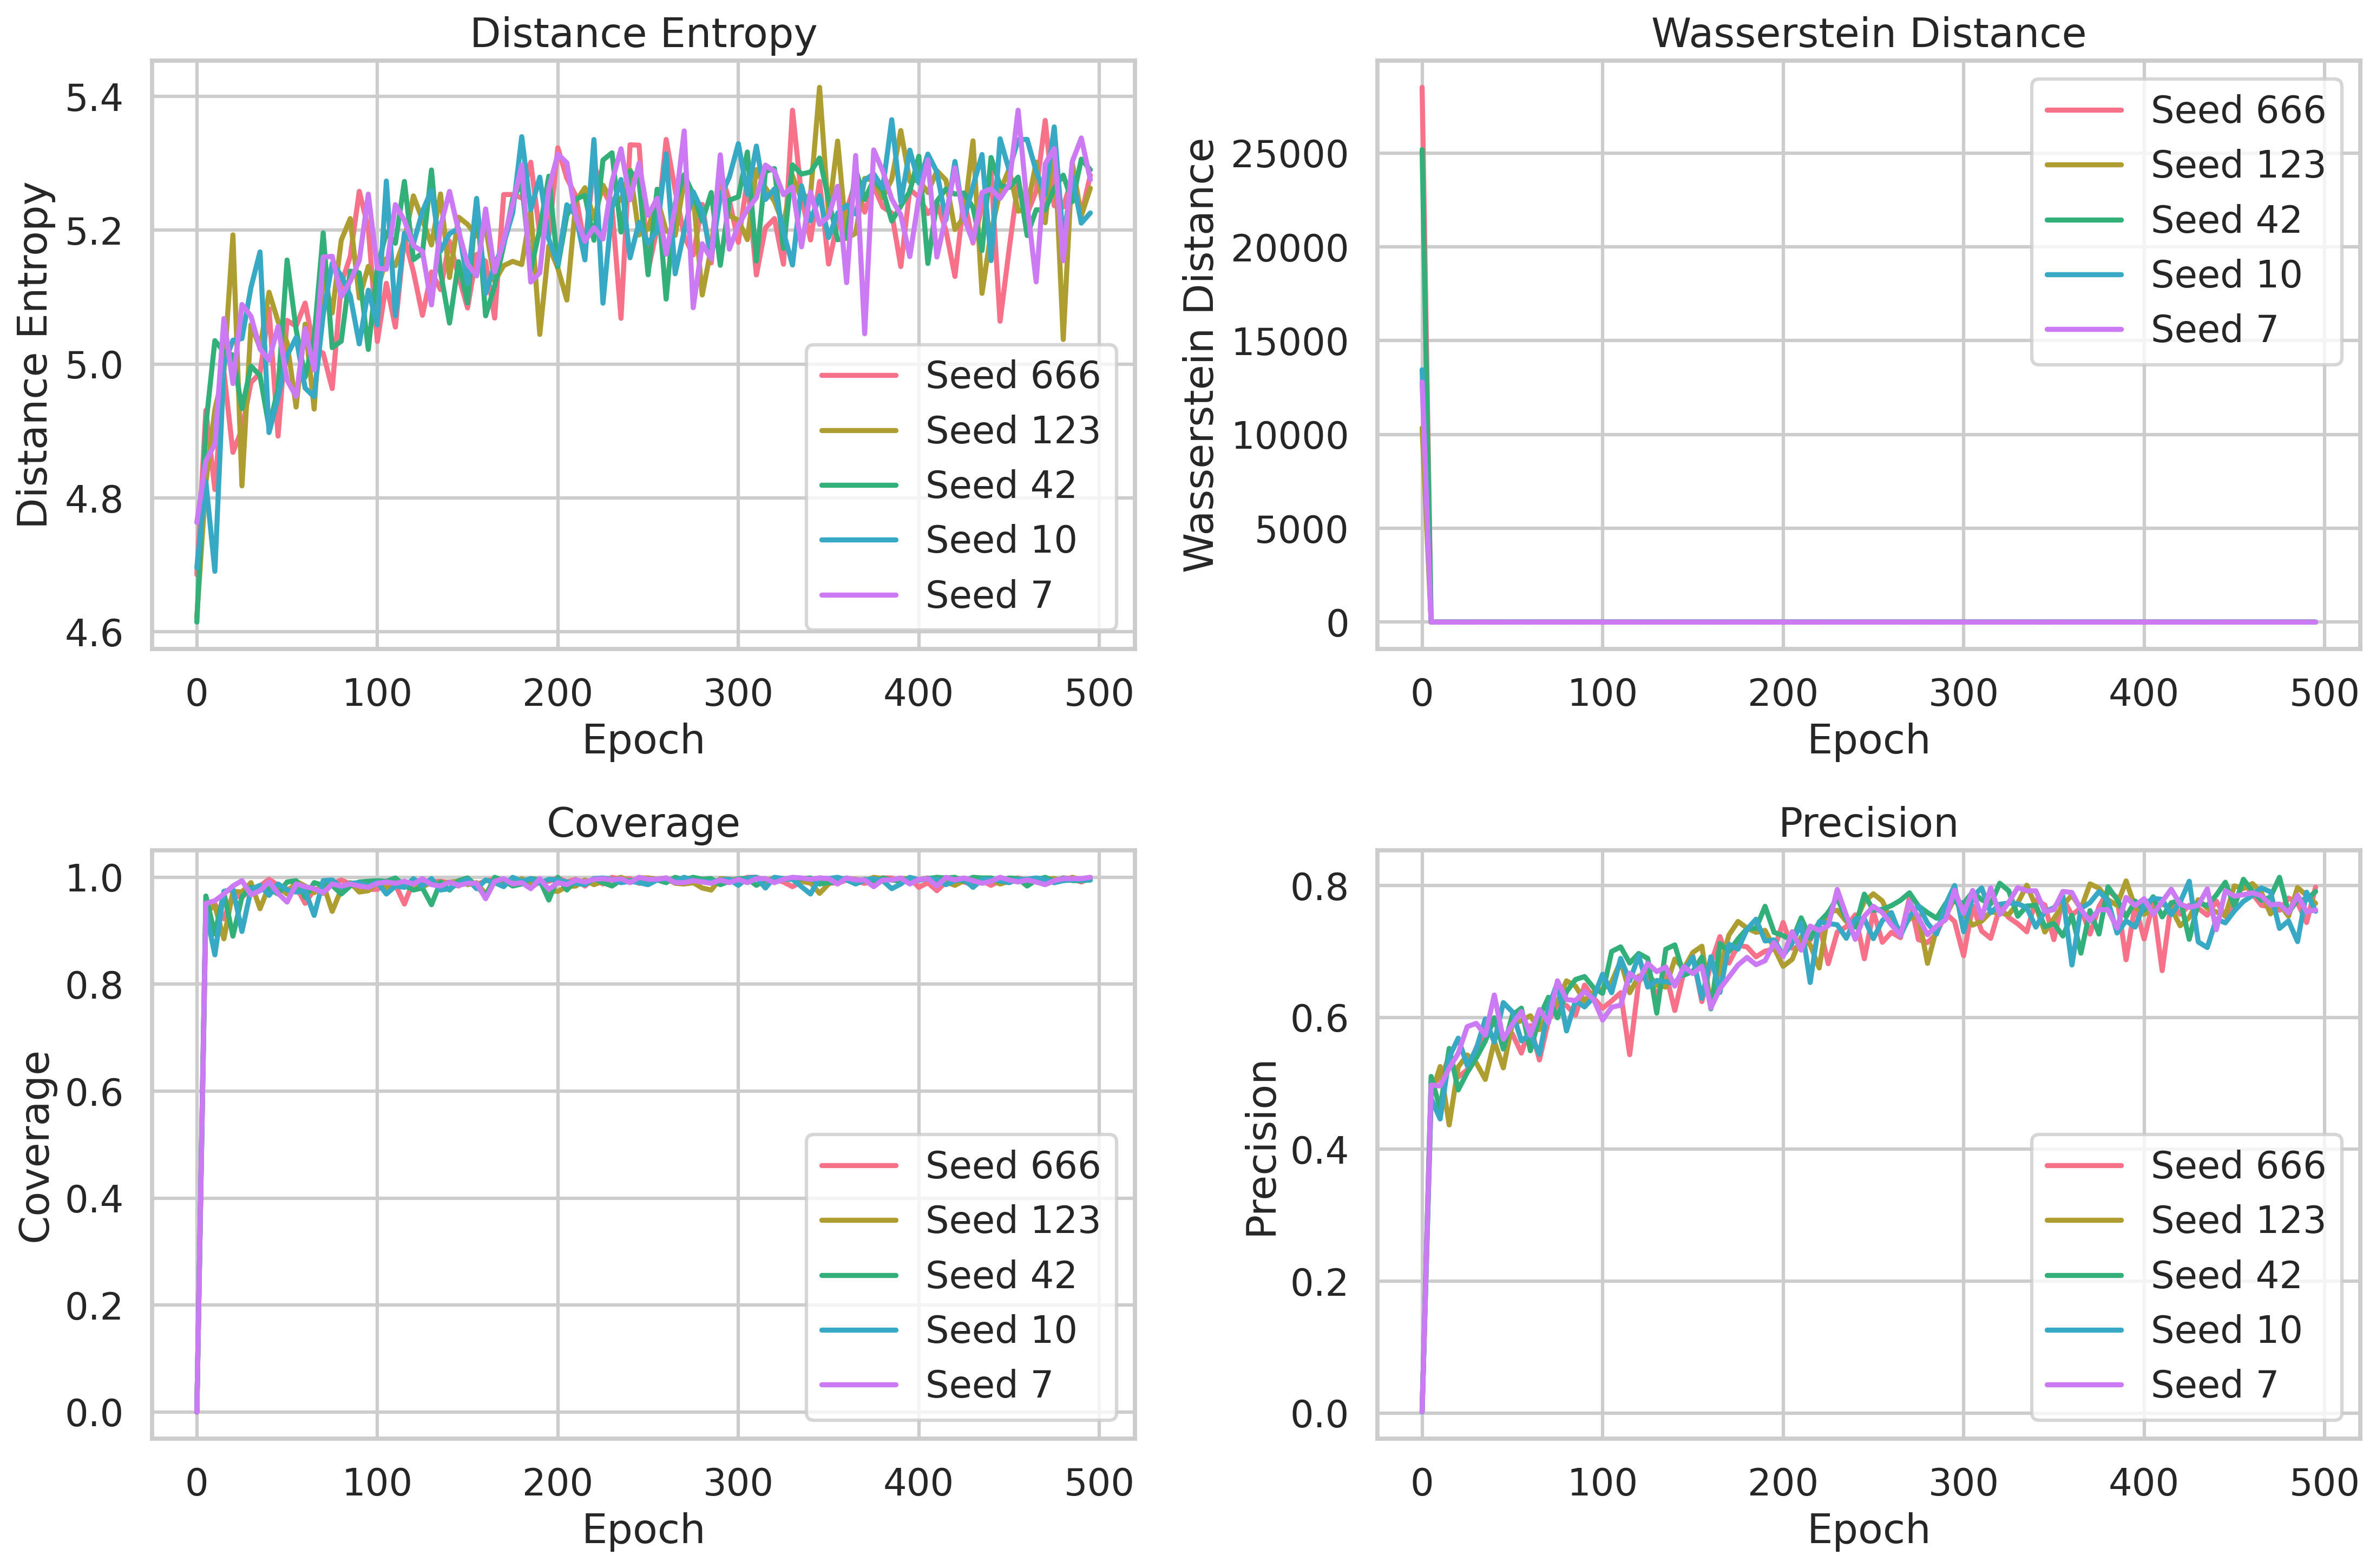
\includegraphics[width=\linewidth]{images/multiseed/diffusion_two_moons_metrics_comparison_optimized}
    \caption{Metric evolution for diffusion on the two moons dataset with optimized hyper parameters.}
    \label{fig:diffusion_two_moons_metrics_comparison_optimized}
\end{figure}

\begin{figure}[tb]
    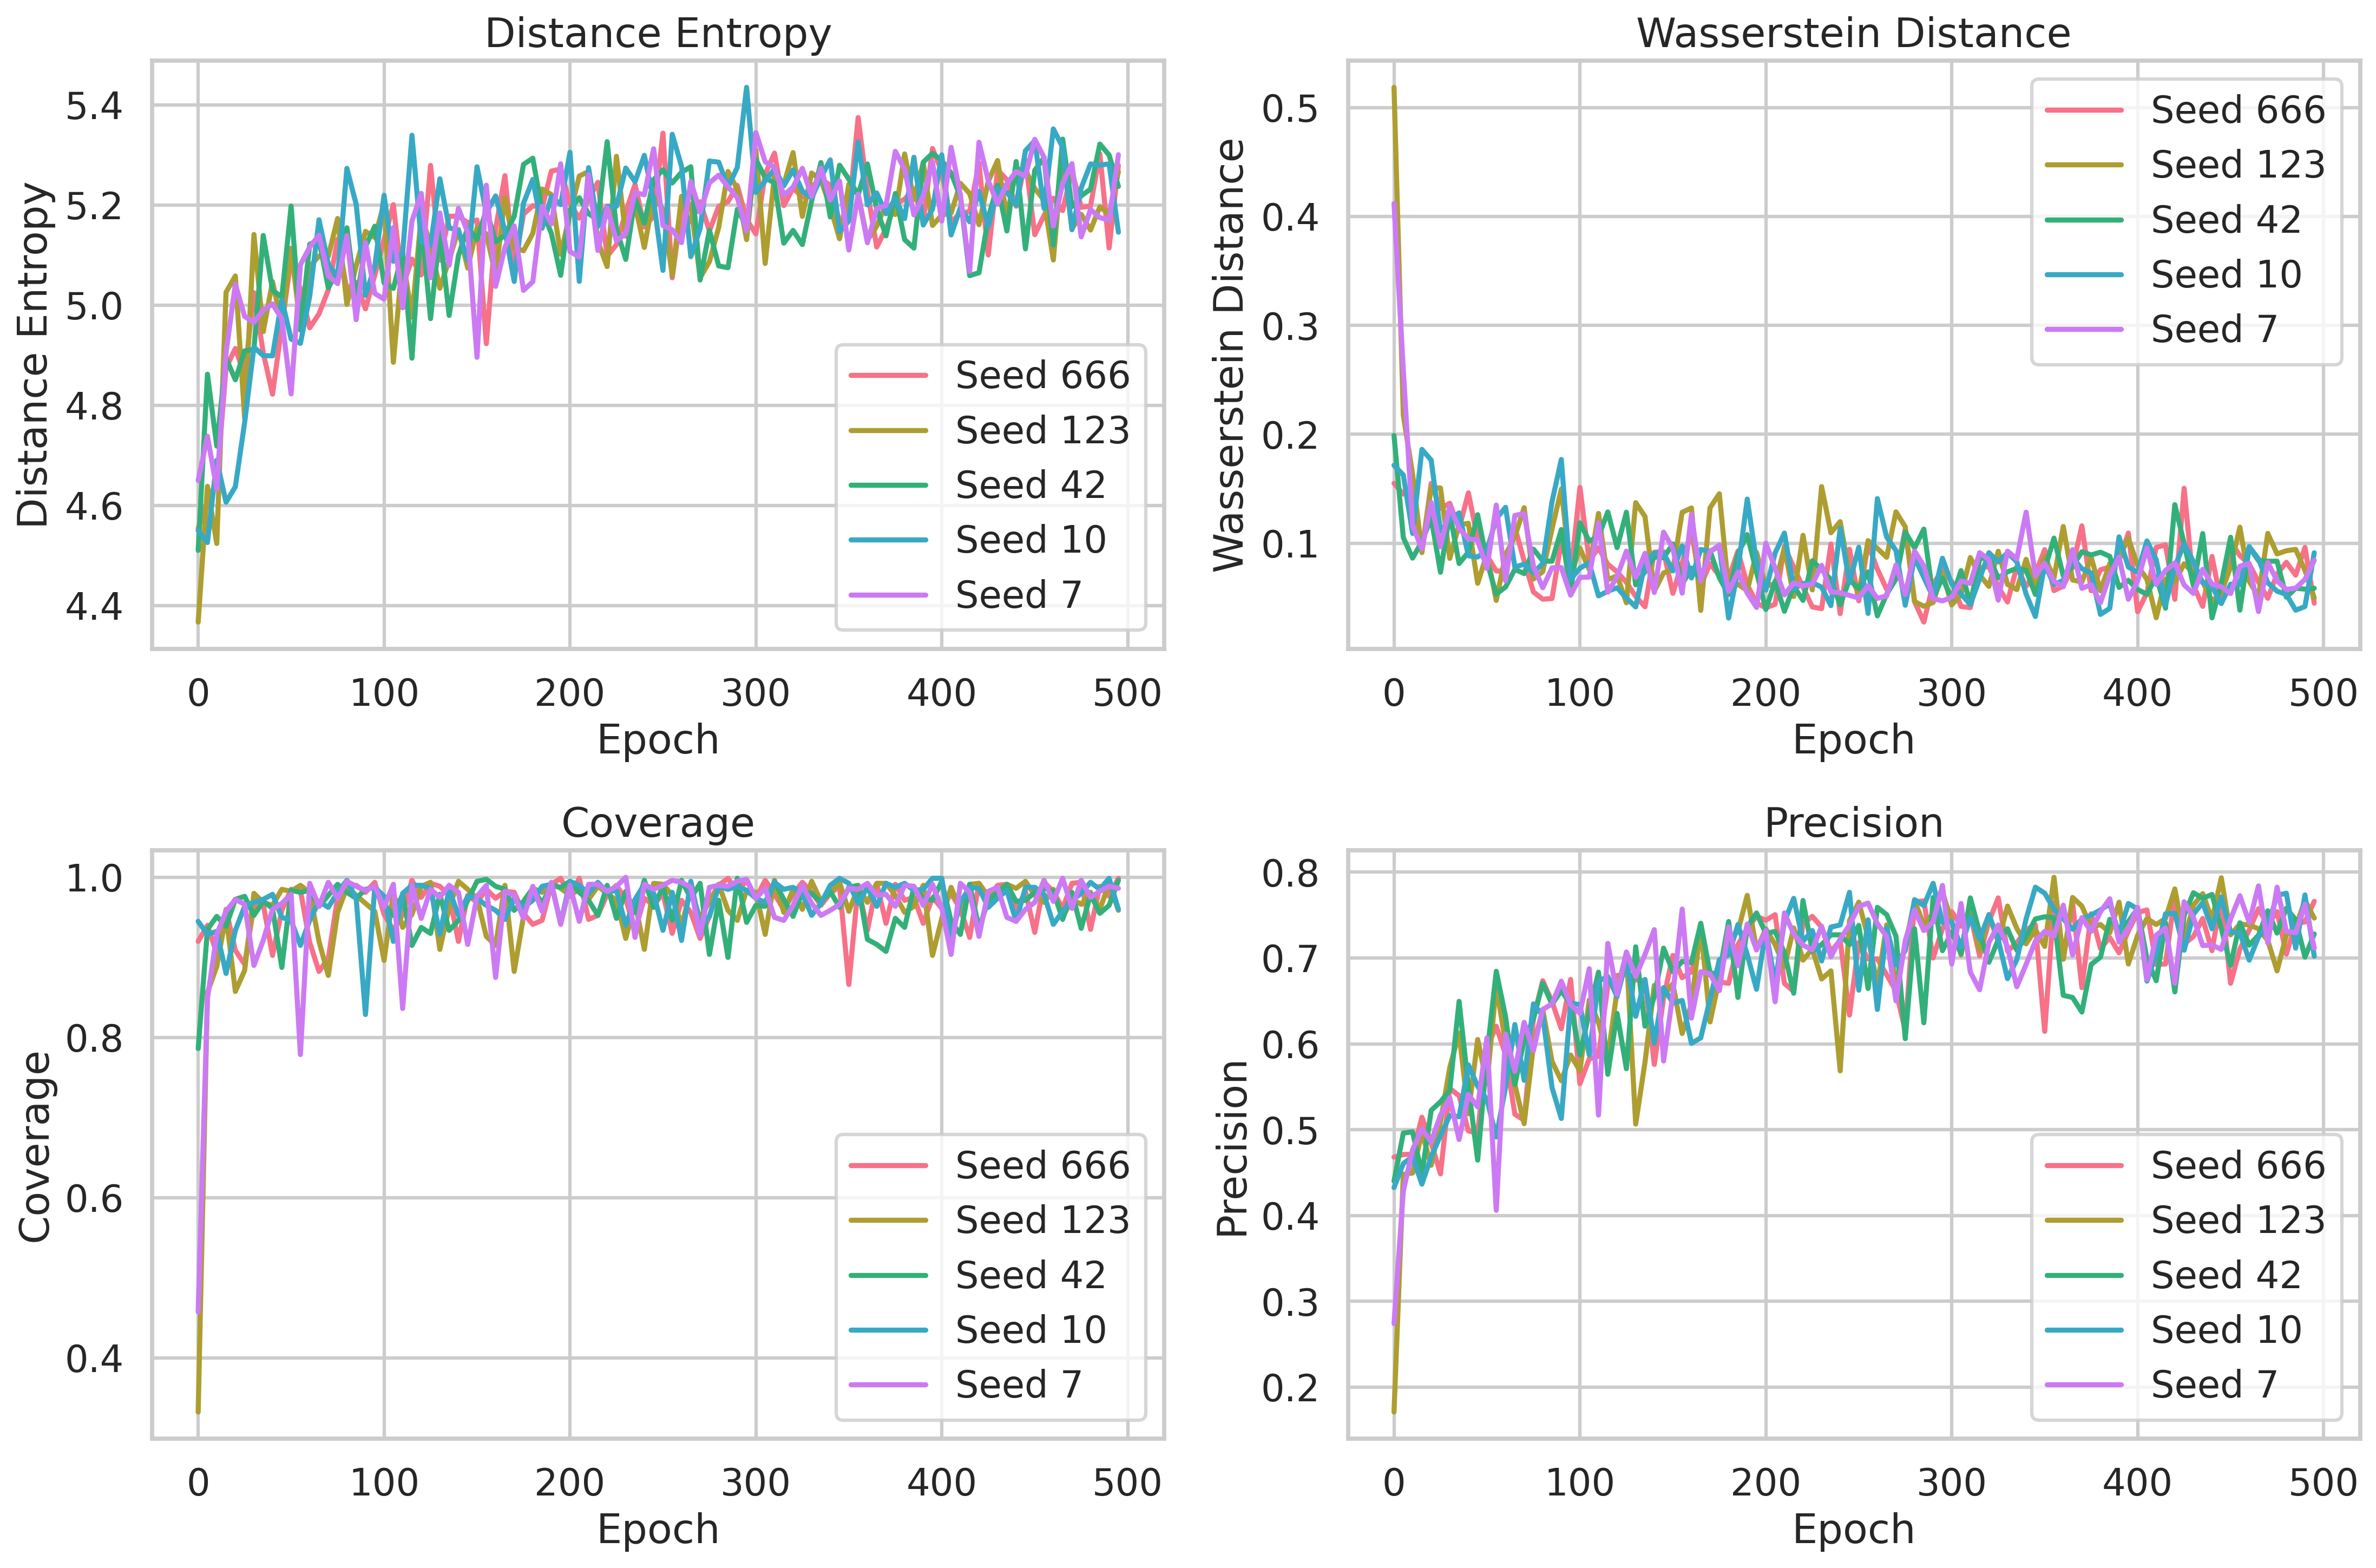
\includegraphics[width=\linewidth]{images/multiseed/flow_matching_two_moons_metrics_comparison_optimized}
    \caption{Metric evolution for flow matching on the two moons dataset with optimized hyper parameters.}
    \label{fig:flow_matching_two_moons_metrics_comparison_optimized}
\end{figure}

\bibliographystyle{plainnat}
\bibliography{references}

\end{document}
